\documentclass[a4paper, 12pt]{article}

% Layout
\usepackage{geometry}
\geometry{left=30mm}
\geometry{right=15mm}
\geometry{top=20mm}
\geometry{bottom=20mm}

% Paragraph
\usepackage{indentfirst}
\setlength{\parindent}{0.75cm}
\linespread{1.25}

% Font
\usepackage{fontspec}
\usepackage[english,russian]{babel}
\usepackage{microtype}

% \usepackage{polyglossia}
% \setmainlanguage{russian}
% \setotherlanguage{english}

% \newfontfamily{\cyrillicfont}{Droid Serif}
% \newfontfamily{\cyrillicfontrm}{Droid Serif}
% \newfontfamily{\cyrillicfontsf}{Droid Sans}
% \newfontfamily{\cyrillicfonttt}{DejaVu Sans Mono}

\setmainfont{Droid Serif}
\setromanfont{Droid Serif}
\setsansfont{Droid Sans}
\setmonofont{DejaVu Sans Mono}

% Hyphens
\usepackage{hyphenat}
\usepackage{ucharclasses}
\setTransitionsForLatin{\begingroup\hyphenrules{english}}{\endgroup}

% Formulas
\usepackage{amssymb, amsfonts, amsmath}

% Miscellaneous
\usepackage{enumerate}
\usepackage{float}
\usepackage{multirow}

% Hyper references
\usepackage{hyperref}
\hypersetup{
    hidelinks,
    allcolors=black
}

% Images
\usepackage{graphicx}
\graphicspath{ {images/} }

%Including title
\usepackage{pdfpages}

% Figures
\usepackage{chngcntr}
\counterwithin{figure}{section}
\usepackage{subcaption}
\renewcommand\thesubfigure{\asbuk{subfigure})}
\captionsetup[subfigure]{labelformat=simple, labelsep=space}

% Counters
\usepackage[figure,table,page]{totalcount}
\usepackage{totcount}

% Code listings
\usepackage{listings}
\usepackage{xcolor}

\definecolor{codegreen}{rgb}{0,0.6,0}
\definecolor{codepurple}{rgb}{0.58,0,0.82}
\lstdefinestyle{codestyle}{
    commentstyle=\color{codegreen},
    keywordstyle=\color{magenta},
    stringstyle=\color{codepurple},
    basicstyle=\ttfamily\footnotesize,
    breakatwhitespace=false,
    breaklines=true,
    captionpos=b,
    keepspaces=true,
    showspaces=false,
    showstringspaces=false,
    showtabs=false,
    tabsize=2
}

\bibliographystyle{gost780s}



\newtotcounter{citenum} %From the package documentation
\def\oldbibitem{}
\let\oldbibitem=\bibitem
\def\bibitem{\stepcounter{citenum}\oldbibitem}

\begin{document}
\includepdf[pages={1}]{title.pdf}

\tableofcontents
\newpage
\section{Введение}
DNS--сервер (Domain Name System) является одной из ключевых составляющих сети Интернет. Он выполняет функцию перевода доменных имен в IP--адреса,
что позволяет пользователям использовать удобочитаемые адреса вместо числовых идентификаторов для доступа к ресурсам в сети. DNS--серверы играют
важную роль в обеспечении стабильной и безопасной работы интернет-инфраструктуры, поэтому их изучение и оптимизация имеют большое значение для
специалистов в области информационных технологий.

Для исследования процесса его работы удобно использовать \textbf{очередь}. В данном случае для задачи имитации сервера об очереди будет рассуждать как
о структуре с доступом к элементам по принципу "первый вошел --- первый вышел" (поскольку при поступлении на сервер запросы обрабатываются в том порядке
, в котором они поступали). Тем не менее, любое цифровое устройство ограничено запасом памяти.

В данной курсовой работе моделирование работы сервера и его ограничение по памяти будет производиться за счет двух очередей: одна будет
представлять сам сервер, обрабатывающий запросы, а вторая --- жесткий диск, на который запросы отправляются в том случае, если они поступили на сервер в момент,
когда очередь обработки на нем переполнена.

Целью данной курсовой работы является определение оптимальной пропускной способности для очереди на сервере в зависимости от интенсивности запросов в
один из трех условных периодов дня: ночь (00:00 -- 9:00), день (9 -- 17:00) и вечер (17:00 -- 00:00).

В ходе работы необходимо решить следующие задачи:
\begin{enumerate}
    \item Поставить задачу, которая позволила бы построить модель для исследования пропускной способности сервера
    \item Построить имитационную модель и провести эксперименты с среде моделирования AnyLogic
    \item Сделать выводы, основываясь на проведенных экспериментах
\end{enumerate}

\newpage
\section{Постановка задачи}
Для проведения эксперимента поставим задачу следующим образом.

На DNS сервер поступают запросы. Длины запросов имеют равномерное распределение с нижней границей
в 10 и верхней в 500 байт. Одновременно в канал сервера может поступать А запросов в секунду. Обработка одного
запроса занимает С миллисекунд. Для необработанных запросов создается очередь, которая записывается
на жесткий диск сервера емкостью B байт. Интенсивность запросов меняется в зависимости от времени суток:
\begin{itemize}
    \item День: в среднем D зап./с
    \item Вечер: V зап./с
    \item Ночь: N зап./с
\end{itemize}

При этом N < D < V. Компьютер клиента может ожидать ответ на запрос в течение 30 секунд.

Задача: определить оптимальную пропускную способность А . Пропускная способность считается оптимальной, когда она минимальна, при условии,
что диск занят не более чем на 70 процентов. Максимальная вместимость диска 500 * 1000 / C * 30  байт.

\subsection{Блок--схема представления модели}

\begin{figure} [h]
    \center{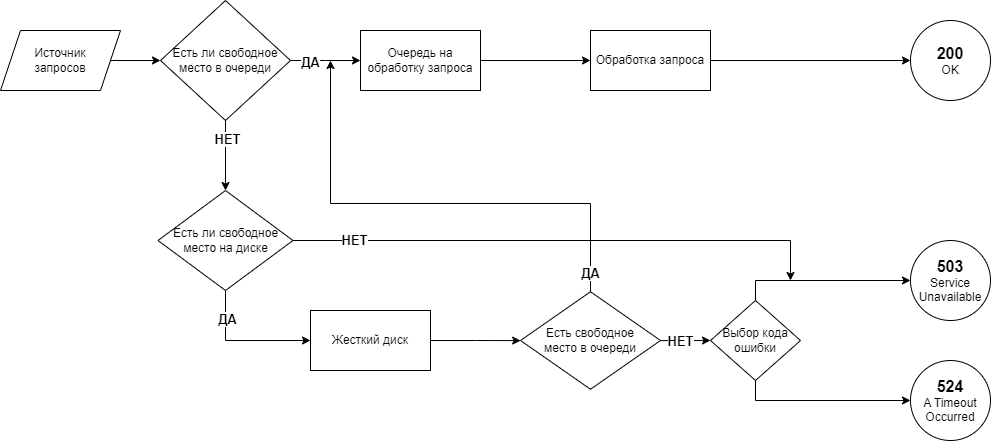
\includegraphics[width=0.9\linewidth]{concept.png}}
    \caption{Логическая блок--схема разработанной модели}
\end{figure}

\newpage
\section{Создание модели в среде AnyLogic}
\begin{figure} [h]
    \center{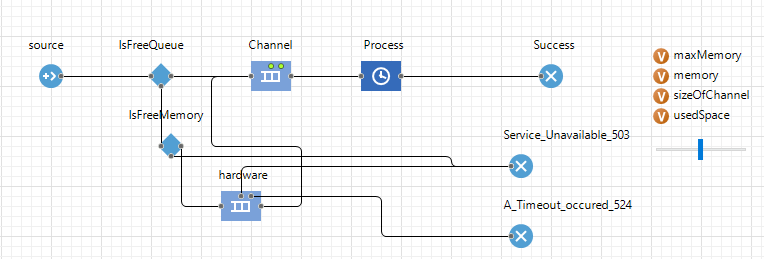
\includegraphics[width=0.9\linewidth]{model.png}}
    \caption{реализация разработанной модели DNS--сервера в среде AnyLogic}
\end{figure}


\subsection{Описание семантики и логики элементов, использованных в модели}

\subsection{Вспомогательные элементы}
Для задания некоторых параметров модели и проведения экспериментов в модели использовались следующие вспомогательные элементы:
\begin{enumerate}
    \item Переменная \textit{maxMemory} --- переменная, необходимая для возможности динамически задавать максимальный размер жесткого диска (
    максимальный размер ЖД был сделан динамическим в целях упрощения проведения серий экспериментов, чтобы не приходилось задавать его вручную
    в зависимости от интенсивности, в момент проведения каждого эксперимента maxMemory является фиксированной величиной)
    \item Переменная \textit{memory} --- переменная, отражающая количество оставшегося места на диске с учетом пришедшего в него на очередь запроса.
    \item Переменная \textit{sizeOfChannel} --- переменная, описывающая искомую величину --- пропускную способность сервера.
    \item Переменная \textit{usedSpace} --- переменная, которая описывает занятое место на диске с учетом пришедшего запроса.
    \item Агент \textit{Запрос} --- транзакт, играющий роль запроса и содержащий информацию о размере этого запроса в байтах.
\end{enumerate}

\subsection{Элементы визуализации}

\newpage
\section{Имитационный эксперимент}

\newpage
\section{Заключение}



\end{document}